\documentclass{standalone}
\begin{document}
\subsection{Pre-processing}

This preliminary step is performed before the training and segmentation process.
It involves the application of the non-local means algorithm to remove possible noise sources and a gamma correction to improve the image contrast.\\
First of all, the MRI scans are acquired from the dataset, slice by slice, in DICOM format and converted into pixel arrays with the original pixel depth in order to preserve all the original information.
Then, to have pixel data in the range $ [ 0, \: 1 ] $, images are normalized and rescaled to binary floating point 32-bit.
This is required to work with \textsc{TensorFlow}\cite{Tensorflow} and \textsc{Keras'} \cite{Keras} functions that deal with the segmentation process, as you will see in the implementation section.
\\
The images are then filtered by using the non-local means algorithm.
In Figure \ref{noisydenoised}, you can see the an example of application of the non-local means algorithm on the same MR image of a patient affected by colorectal cancer.
The original image on the \textit{left}, is affected by noise while the filtered one, on the \textit{right}, results smoothed without significant detail loss. 
In fact, one drawback of smoothing filters is the blurring of small details but in this case, they are preserved.
This behavior is reflected in the image histogram. 
As you can see in Figure \ref{histo}, the original image histogram (red) is affected by great fluctuations of pixel intensity, that highlight the presence of noise. 
Instead, the denoised image histogram (blue) results in a smoothed histogram, preserving the original shape.
\\
After performing the non-local means algorithm, the image contrast is enhanced by a gamma correction.
In this case, the $\gamma$ parameter has been set to a value of 1/1.5 to make darker regions lighter.
An example of the performed gamma correction can be seen in Figure \ref{denoisedgamma}.
Moreover, the rise of contrast can be noticed on the gamma-corrected image histogram, shown in Figure \ref{histogamma}.
\\
In summary, the preprocessing steps are:
\begin{itemize}
    \item normalization and rescaling
    \item denoising
    \item gamma correction
\end{itemize}

A comparison of the image before and after the pre-processing can be seen in Figure \ref{noisyfinal}.

\begin{figure}[htp]

    \centering
    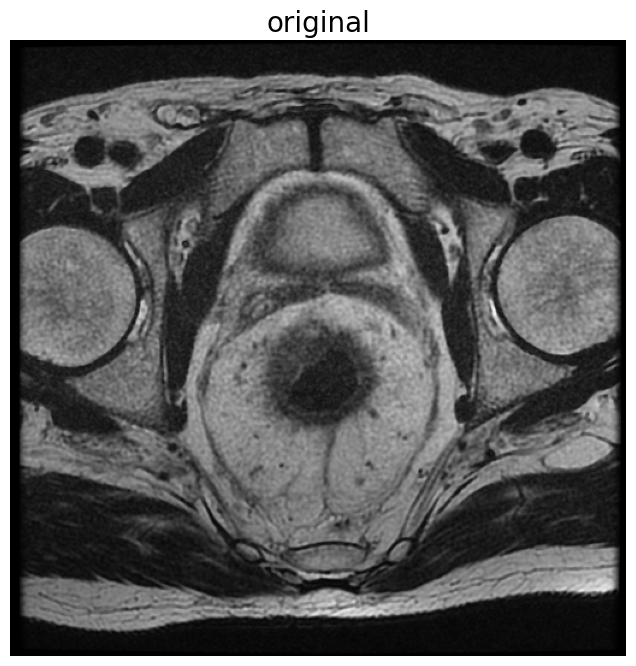
\includegraphics[width=.49\textwidth]{../images/noisy.png}
    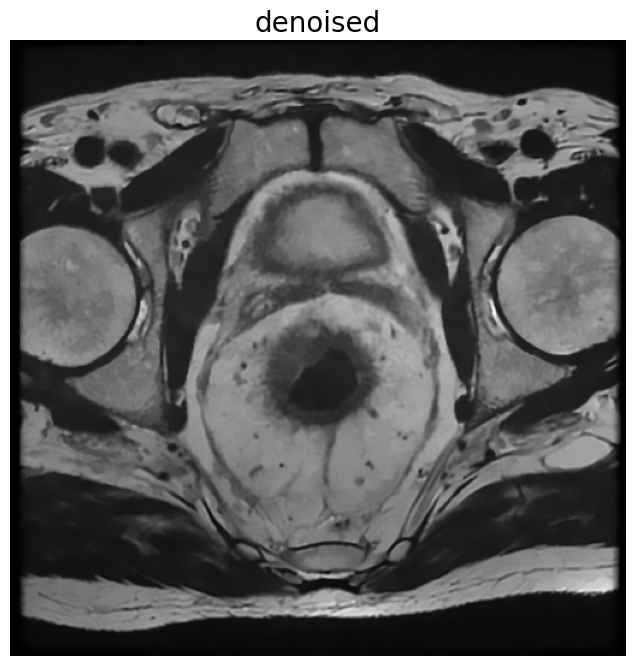
\includegraphics[width=.49\textwidth]{../images/denoised.png}
    
    \caption{ \textit{ Left)} Original MR image of a patient affected by colorectal cancer.\textit{ Right)} The same image after non-local mean algorithm.}
    \label{noisydenoised}
    
    \end{figure}

\begin{figure}[htp]

    \centering
    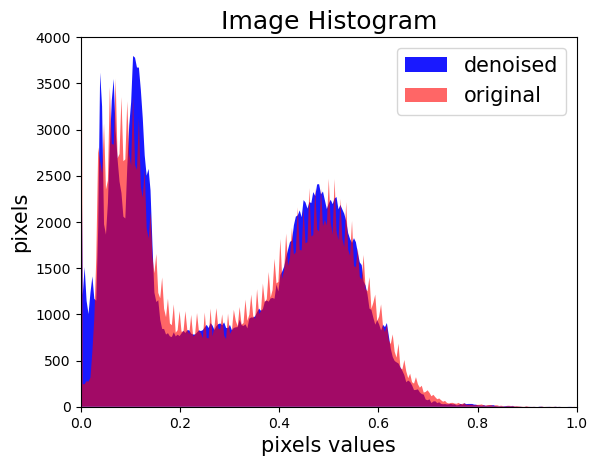
\includegraphics[width=0.73\textwidth]{../images/histogram.png}

    
    \caption{Original vs denoised image histogram. The original image histogram (red) is affected by great fluctuations of pixel intensity, highlighting the presence of noise. The denoised one (blue) results in a smoothed histogram, preserving the original shape.}
    \label{histo}
    
    \end{figure}

\begin{figure}[htp]

    \centering
    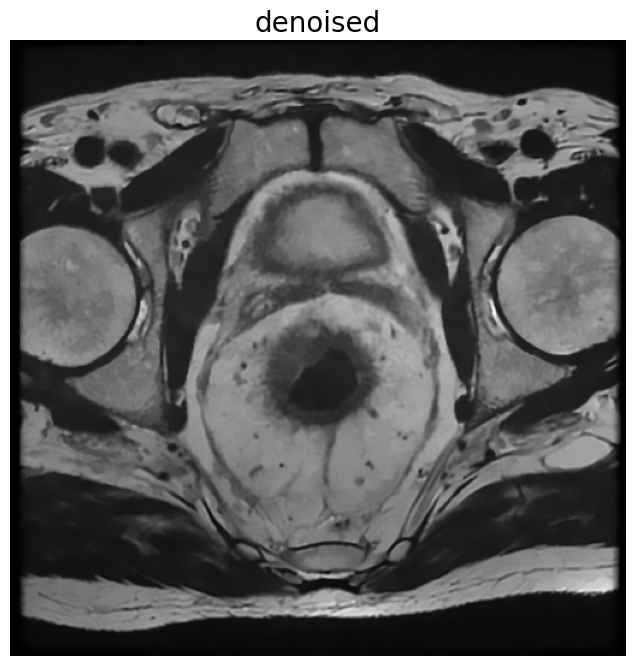
\includegraphics[width=.49\textwidth]{../images/denoised.png}
    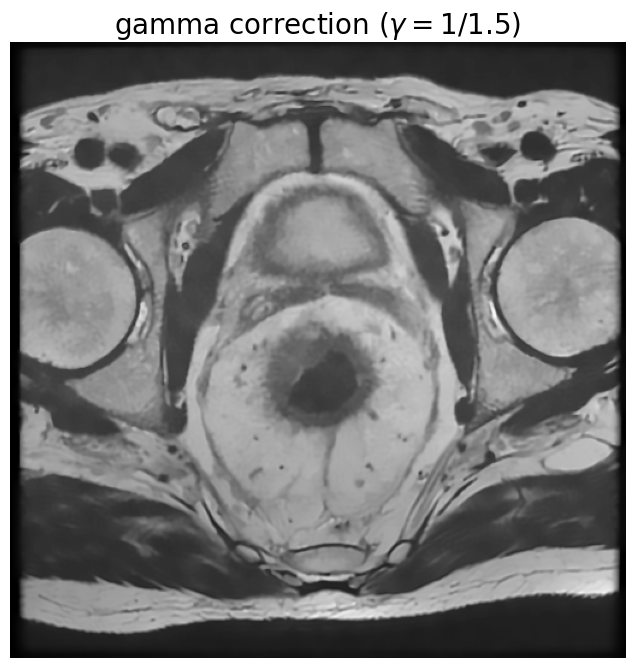
\includegraphics[width=.49\textwidth]{../images/gammacorrection.png}
    
    \caption{ \textit{ Left)} denoised MR image of a patient affected by colorectal cancer.\textit{ Right)} The same image after gamma correction.}
    \label{denoisedgamma}
    
    \end{figure}

\begin{figure}[htp]

    \centering
    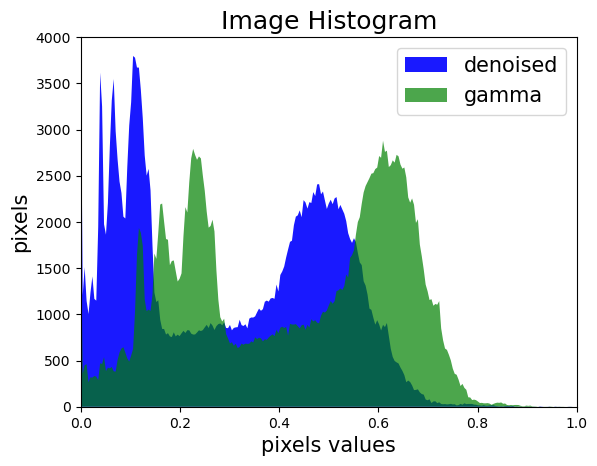
\includegraphics[width=0.73\textwidth]{../images/gammahist.png}

    
    \caption{Denoised vs gamma-corrected image histogram. The gamma-corrected image histogram (green) results in a right-shifted histogram.}
    \label{histogamma}
    
    \end{figure}

\begin{figure}[htp]

    \centering
    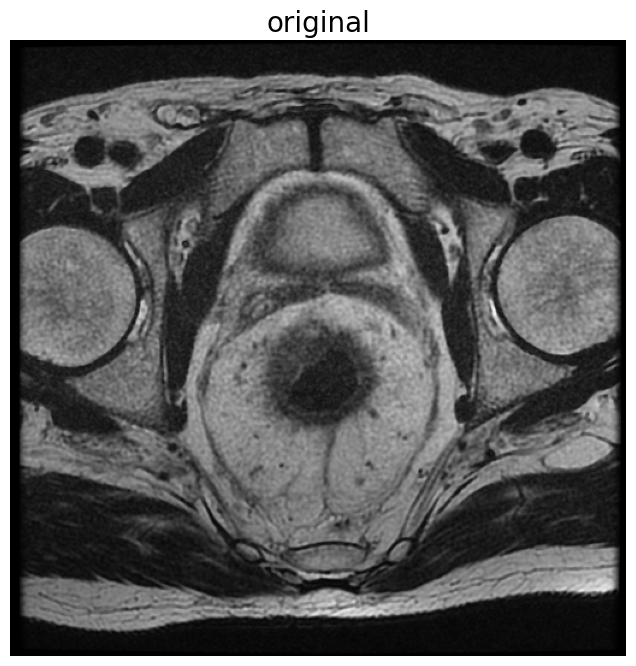
\includegraphics[width=.49\textwidth]{../images/noisy.png}
    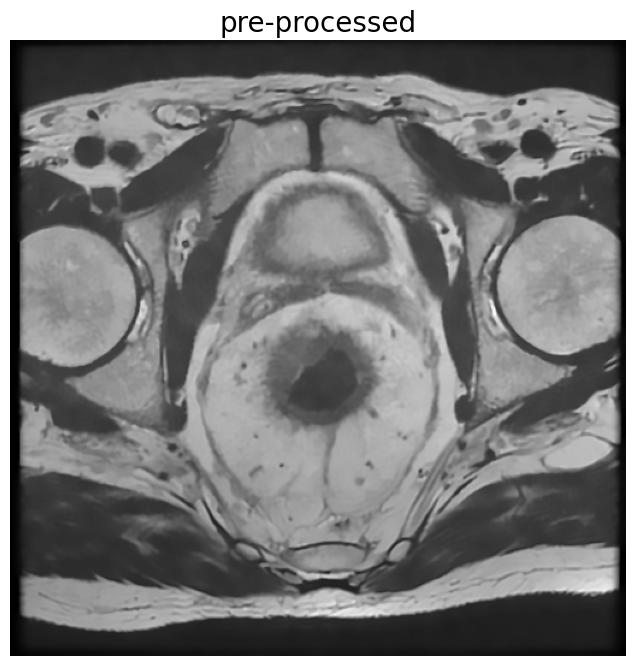
\includegraphics[width=.49\textwidth]{../images/finalimage.png}
    
    \caption{ \textit{ Left)} Original MR image of a patient affected by colorectal cancer.\textit{ Right)} The same image after the pre-processing steps.}
    \label{noisyfinal}
    
    \end{figure}
\end{document}